%
% LogMon Manual
%

\documentclass[11pt,a4paper]{article}

\setlength{\parskip}{1.1ex}
\setlength{\parindent}{0em}

\setlength{\oddsidemargin}{0cm} %now 1in
\setlength{\textwidth}{17cm}
\setlength{\textheight}{22cm}

\usepackage[utf8]{inputenc}
\usepackage{graphicx}

\title{LogMon Manual}
\author{Thomas Weidlich}

%Create a brand :-)
\newcommand{\logmon}{\textbf{LogMon\ }}

%some other brand
\newcommand{\js}{\textit{JavaScript\ }}
\newcommand{\java}{\textit{Java\ }}

\begin{document}

\maketitle
\tableofcontents
\newpage
%---------------------------------------------------------------------------------------------------------------
\section{Introduction}

\logmon is a simple logfile monitor written in \java. The main features are:

\begin{itemize}
  \item Use regex
  \item Modular escalation
  \item Local correlation in \js
  \item Configuration in single xml file
  \item No installation
  \item Store last reading position
\end{itemize}

\logmon allow the usage of \js to decide a escalation. Add a
\verb#<condition># tag in each \verb#<pattern># tag to define the script name.
The \js will run on every time where the pattern match.

%---------------------------------------------------------------------------------------------------------------
\section{Installation}

Simply copy logmon.jar and one alert module jar in a folder. Create a
configuration file and start \logmon with \java version 6 or later. If the
alert module require some additional jar, copy also into the folder.

\begin{verbatim}

java -cp logmonModMail.jar:logmon.jar:lib/mail.jar \
    app.LogMon --config=config.xml

\end{verbatim}

%---------------------------------------------------------------------------------------------------------------
\section{The configuration}
\label{sec:conf}

\logmon require one (validated) xml file for configuration. Use argument
 \verb#--config=filename.xml# to set file.
There are three section inside of configuration file. See chapters blow for documentation.

\begin{itemize}
  \item database
  \item alert
  \item logfiles
\end{itemize}

\subsection{The section: database}
\label{sec:cfgdb}

The database section set name and path of internal database files. The database files store events for
correlation from \js and last reading positions. The path entry is optional. If not set, the current working
directory is used. Examples:

\begin{verbatim}
  <database>
      <id>LinuxBase</id>
      <path>/tmp</path>
  </database>
\end{verbatim}

\subsection{The section: alert}

The way-of-alert is set in alert section. You have to add one alert module to \java \textit{classpath}
and setup the alerting in alert section. Today are two alert modules available:

\bigskip
\begin{tabular}{ll}
  Mail 	     & logmonModmail.jar\\[1ex]
  Tivoli TEC & logmonModEIF.jar\\
\end{tabular}
\bigskip

See modules chapter at page \pageref{sec:modules} for additional alert
configuration entry's. At this point a simple example

\begin{samepage}
\begin{verbatim}

<alert>
    <class>mon.evt.StdoutAlert</class>
    <properties>
        <property name="init.msg"></property>
        <property name="send.pre">ERROR></property>
    </properties>
</alert>

\end{verbatim}
\end{samepage}

To implement more alert modules you need \java Known-How and the alert interface
from logmon source.

\subsection{The section: logfile}

The most important part of configuration are the one or more sections \verb#<logfile>#. You can
setup one or more logfiles with different pattern definitions! One first simple minimal example:

\begin{samepage}
\label{ex:logfile1}
\begin{verbatim}
  <logfile>
    <file start="begin">test.log</file>
    <pattern>
      <regex>.*Error(.*)</regex>
      <msg>Error: $1</msg>
      <severity>CRITICAL</severity>
    </pattern>
  </logfile>
\end{verbatim}
\end{samepage}

The first entry below \verb#<logfile># is the \verb#<file># entry to describe
the logfile path. You can use environment variables in perl syntax
\verb#$ENV{HOME}/myfile.log#. The attribute start set the reading-start-position
of logmon. You can use BEGIN or CURRENT or LAST.
After the \verb#<file># section
follow one more \verb#<pattern># definitions. Each \verb#<pattern># require the
three child \verb#<regex>#, \verb#<msg># an \verb#<severity>#. Optional there
are one \verb#<condition># and one \verb#<properties># child.

The \verb#<regex># contain a regular expression with or without groups. The
matched group values available in \verb#<msg># as \$1 for first group and \$2
for second group and so on. The groups also available in conditions scripts. See
description blow.

The resolved \verb#<msg># will send to alert receiver. You can use groups from
regular expression and environment variables in perl syntax. The resolved message
is changeable from condition script.

The valid severity's are INFO,WARNING,MINOR,CRITICAL.

The next example at page \pageref{ex:logfile2} a additional child
\verb#<condition>#. It set the filename of some \js file. This file will
call on every match of this pattern. If a condition script is given the alert
is only send if the pattern matches \textbf{and} the condition script return
\verb#status=true#. See chapter \ref{sec:conditions}

If no condition script is given the alert will send every time the pattern
match.

The next optional child of \verb#<logfile># is \verb#<properties>#. You can
change every init and send property of \textbf{this} alert.

\begin{samepage}
\label{ex:logfile2}

\begin{verbatim}
<logfile>
  <file start="current">/var/log/messages</file>
  <pattern>
    <regex>(\w+)\s+(\d+)\s+([\d:]+).*Deny Policy.*SRC=([\d\.]+).*DPT=(\d+)</regex>
    <msg>Firewall deny from IP $4 to Port $5</msg>
    <severity>WARNING</severity>
    <condition>firewall.js</condition>
  </pattern>
  <pattern>
    <regex>.*Error(.*)</regex>
    <msg>Error: $1</msg>
    <severity>CRITICAL</severity>
    <properties>
        <property name="send.smtp.subject">Error from Logfile</property>
    </properties>
  </pattern>
</logfile>
\end{verbatim}
\end{samepage}

%---------------------------------------------------------------------------------------------------------------
\section{Condition scripts}
\label{sec:conditions}

The condition script allow a local correlation of logfile entry's before
see alert to any receiver. You can send only every 5 entry for example or send only
if some other entry was found in the past. Or you send only if more then 10 match
in 2 hour. The condition script are written in \js and run every matched line.
the value of the variable \textit{status} decide to send alert. If the \js
set \textit{status=true}, the alert will send. You can use every \js code
inside. You have for,while,if and so one. There are some variables and instances
already set by \logmon.

\begin{table}[ht]
\begin{tabular}{l|l|p{0.5\textwidth}}

  Name & Type & Description\\\hline\hline

  pattern & String &
  The matched regular expression (Readonly) \\\hline

  logline & String &
  The current line from logfile. (Readonly)\\\hline

  status & String &
  The script return status. Default is false. If set to true
  the alert method will call\\\hline

  msg & 	String &
  The resolved messages. The script can change it.\\\hline

  db & Object &
  Database connection with method db.save(id) and db.load(id).
  Both method use/change/update the  variable occurrence\\\hline

  occurrence & 	Object &
  The occurrence instance contains the attributes
  created,modified,maxage,repeat and groups. See Occurrence description\\\hline

\end{tabular}
\label{tab:vars}
\caption{Internal variables and instances}
\end{table}

The simple thing first: The variable \textit{pattern} and \textit{logline}
are read only and contain the \verb#<regex># from configuration and the
current matched line from logfile. The \textit{msg} contain the resolved
message from configuration with all groups from \verb#<regex>#. You
can change it inside of \js. The \textit{status} is set to \textit{false}
and only if the \js code change it to \textit{true} the alert will send!

OK, lets got to next level. The next entry in table is the db instance
with method \textit{save(\textless{}id\textgreater{})}, \textit{load(\textless{}id\textgreater{})}
and \textit{remove(\textless{}id\textgreater{})}. This three method are the interface to
a small database for store \textit{occurrence} instance. A \textit{occurrence} instance is created
on every time a regex matched and you can save it inside the database. If a entry with same
 id already exists it will updated. The repeat will increase, the modified time is changed and
 the groups[] is change to current match. If the current time is greater (later) then
 created+maxage (default 7 days) the entry is remove automatic, but you can remove every time.
 All condition scripts can access \underline{all} database entry's by select the
 entry id's.

\begin{table}[ht]
\begin{tabular}{l|p{0.5\textwidth}}
  Attribute & Description\\\hline\hline
  created   & Epoch second of creation\\\hline
  modified  & Epoch second of last modified\\\hline

  maxage    & Maximal seconds store in database. The database entry will remove
  if \verb# created+maxage > now#\\\hline

  repeat    & The repeat count is increased while every db.save(id)
  action\\\hline

  groups[]  & String array of all matched groups from regex. The index start
  with 0 (zero)!!\\\hline
\end{tabular}
\caption{The occurrence object}
\label{tab:occurr}
\end{table}

The used database is in memory but there is a mirror one file-system. The name and path are give in first
section in configuration file. See chapter \ref{sec:cfgdb}. It is a simple CSV file but you can't change
it while \logmon is running!

Now let's look one first example. The follow example look for firewall line on a
Linux system. The regex from configuration is
\verb#(\w+)\s+(\d+)\s+([\d:]+).*Deny Policy.*SRC=([\d\.]+).*DPT=(\d+)# and you
see the fourth (index 3!!) regex-group contain the IP of the dropped connection.
I use this IP as database index. I change the maxage to 1h check the repeat
counter after saving in db.

The result is: Alert if there more as 5 connection
from same IP in 1 hour then alert every 5 occurrence.

\begin{samepage}
\begin{verbatim}
var src=occurrence.groups[3];
occurrence.maxage=3600;

db.save("FW"+src);

if(occurrence.repeat >=5  && occurrence.repeat % 5 ==0){
        status=true;
}
\end{verbatim}
\end{samepage}

Note the \% is the modulo operation in \js

%---------------------------------------------------------------------------------------------------------------
\section{Modules}
\label{sec:modules}

\subsection{Setting of all modules}

Every module implements a IAlert interface with three method init() send() stop(). All three method
have a Properties instance as argument. The init() method all properties stating with init, the send()
all properties starting with send and the stop() method starting with stop. The table below show
all properties used by all module.  You can set this properties (except send.repeat) inside section \verb#<alert># or inside
section \verb#<pattern># of configuration file.

For module additional properties see chapters below.

\begin{tabular}{l|p{0.5\textwidth}}
  Property 	& Description\\\hline
  send.repeat  	    & The repeat count \\
  send.severity 	& The severity \\
  send.hostname 	& The hostname of problem location\\
  send.msg 	        & The message\\
\end{tabular}

For all \java programmer the interface. For more information see \logmon source.

\begin{samepage}


\begin{verbatim}
package mon.evt;

import java.util.Properties;

public interface IAlert {

  public boolean init(Properties properties);

  public boolean send(Properties properties);

  public boolean stop();
}

\end{verbatim}
\end{samepage}


\subsection{Alert module: STDOUT}

The stdout module alerts to the stdout console. I use it for debugging.

\begin{tabular}{l|p{0.5\textwidth}}
  Property 	& Description\\\hline
  init.msg 	& Show this string at start of logmon\\
  send.pre 	& Show this string at every line\\
\end{tabular}

\begin{verbatim}
  <alert>
    <class>mon.evt.StdoutAlert</class>
    <properties>
      <property name="init.msg">Hello World</property>
      <property name="send.pre">Alert: </property>
    </properties>
  </alert>
\end{verbatim}

\subsection{Alert module IBM Tivoli EIF}
\label{sec:eif}

Send Event to IBM Tivoli Enterprise Console. It require some additional jar in
folder lib. Contact IBM and ask for EIF SDK. The most important the properties
init.tec1 and init.tec2. Setup two ``TEC Gateway Reciever'' (most time TEC
servers).

\begin{verbatim}
  <properties>
    <property name="init.tec1">tecgw1.tivoli.net</property>
    <property name="init.tec2">tecgw2.tivoli.net</property>
    <property name="send.class">MY_Event</property>
  </properties>
\end{verbatim}

\subsection{Alert module Mail}

Send alert as mail to SMTP receiver. Require the additional jar mail in
CLASSPATH. If the SMTP server need some authentication set user and
password. Be careful about file permissions of
configuration! This is not a secure setup.

\begin{tabular}{l|p{0.5\textwidth}}
  Property 		    & Description\\\hline
  init.smtp.server 	& The smtp server\\
  init.smtp.from    & Sender mail address\\
  init.smtp.user 	& The user if smtp need authentication\\
  init.smtp.pwd 	& The password if smtp need authentication\\
  send.smtp.to 		& Receiver mail address\\
  send.smtp.subject & The Mail subject\\
\end{tabular}

\section{Debugging}

\subsection{logging}

To write a logfile for debugging create logging.properties file an add
\textbf{-Djava.util.logging.config.file = logging.properties} to arguments.
For more information see \java
logging documentation. Example properties file:

\begin{verbatim}
#
# Add -Djava.util.logging.config.file=logging.properties to vm arguments
#
handlers= java.util.logging.FileHandler,java.util.logging.ConsoleHandler

.level=INFO

#app.level=ALL
#cfg.level=ALL
#mon.level=ALL
#alert.level=ALL

# Setup handlers
java.util.logging.ConsoleHandler.level = INFO

java.util.logging.FileHandler.level=ALL
java.util.logging.FileHandler.formatter=java.util.logging.SimpleFormatter
java.util.logging.FileHandler.pattern=logmon.log
java.util.logging.FileHandler.limit=102400
java.util.logging.FileHandler.count=5
java.util.logging.FileHandler.append=false

\end{verbatim}

\subsection{JMX (\java Management Extensions)}

I add some JMX MBean to \logmon. To monitor \logmon from remote add follow
arguments. It open some port without any security. Be careful!
If you need some secure connection setting, please show \java jmx documentation.

\begin{figure}[h]
\centering
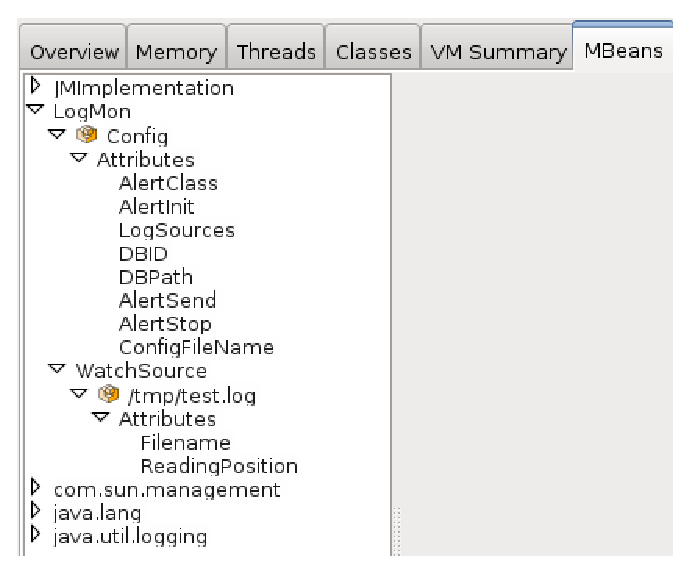
\includegraphics{img/jconsole.eps}
\caption{jconsole}
\end{figure}

\begin{verbatim}
-Djava.net.preferIPv4Stack=true
-Dcom.sun.management.jmxremote
-Dcom.sun.management.jmxremote.port=9494
-Dcom.sun.management.jmxremote.authenticate=false
-Dcom.sun.management.jmxremote.ssl=false
\end{verbatim}

You can use ssh to tunnel the JMX  connecting from your workstation to \logmon
server. First connect to the server by ssh. Add \textit{-D \textless{}some-free-port\textgreater{}  } to ssh.

\begin{verbatim}
ssh -D 9494 myhost.com
\end{verbatim}

Now you start a jmx console at your workstation and connect it to the \logmon
server. For \textit{jconsole} use:

\begin{verbatim}
jconsole -J-DsocksProxyHost=localhost -J-DsocksProxyPort=9494 \
service:jmx:rmi:///jndi/rmi://myhost.com:9494/jmxrmi
\end{verbatim}


Or or \textit{jvisualvm} use:

\begin{verbatim}
jvisualvm \
    -J-Dnetbeans.system_socks_proxy=localhost:9494 \
    -J-Djava.net.useSystemProxies=true
\end{verbatim}

And then:

\begin{itemize}
  \item Add Remote Host ( myhost.com )
  \item Add JMX Connection ( myhost.com:9494 )
\end{itemize}

%--------------------------------------------------------------------------
\appendix

\section{Configuration example files}
\label{sec:confex}

Monitor Linux syslog an send alert to Tivoli TEC:

\begin{verbatim}

<?xml version="1.0" encoding="UTF-8"?>
<!DOCTYPE config SYSTEM "configuration.dtd">
<config>
  <database>
    <id>LinuxTest</id>
  </database>
  <alert>
    <class>alert.Tivoli</class>
    <properties>
      <property name="init.tec1">gateway1.tivoli.net</property>
      <property name="init.tec2">gateway2.tivoli.net</property>
      <property name="send.class">MY_Class</property>
      <property name="send.hostname">MYHOST</property>
    </properties>
  </alert>
  <logfile>
    <!-- Start position at current or begin -->
    <file start="current">/var/log/messages</file>
    <pattern>
      <regex>(\w+)\s+(\d+)\s+([\d:]+).*Deny Policy.*SRC=([\d\.]+).*DPT=(\d+)</regex>
      <msg>Firewall deny from IP $4 to Port $5</msg>
      <severity>WARNING</severity>
      <condition>firewall.js</condition>
    </pattern>
    <pattern>
      <regex>.*Error(.*)</regex>
      <msg>Error: $1</msg>
      <severity>CRITICAL</severity>
      <properties>
        <property name="send.slot.srcip">$1</property>
        <property name="send.slot.appl">Firewall</property>
      </properties>
    </pattern>
  </logfile>
</config>

\end{verbatim}

Monitor logfile and print alert to stdout:

\begin{verbatim}
<?xml version="1.0" encoding="UTF-8"?>
<!DOCTYPE config SYSTEM "configuration.dtd">
<config>
  <database>
    <id>WinTest</id>
    <path>C:\temp</path>
  </database>
  <alert>
    <class>mon.evt.StdoutAlert</class>
    <properties>
      <property name="init.msg"></property>
      <property name="send.pre">ERROR></property>
    </properties>
  </alert>
  <logfile>
    <file start="last">test.log</file>
    <pattern>
      <regex>.*Error:(.*)</regex>
      <msg>Error: $1</msg>
      <severity>WARNING</severity>
      <condition>test.js</condition>
    </pattern>
  </logfile>
</config>
\end{verbatim}

\end{document}

